\graphicspath{{Chapter3/Chapter3Figs/}}


\chapter{mTOR network: an overview}
\label{chap:mTOR network: an overview}
TOR kinase is centrally located in a complex signalling network that responds to the availability of cellular resources. TOR is positively regulated by growth factors, nutrients and energy uptake. Through these signals, the kinase activates protein translation initiation and elongation mechanisms, regulates cell growth and metabolism, improves mitochondria function and transmits signals for cell survival. TOR-activated downstream targets inhibit apoptosis, autophagy and cell cycle arrest. Conversely, nutritional or energetic stress conditions negatively control TOR activity. The TOR network is further complicated by several feedback mechanisms that work at different time-scales and hamper a full understanding. This chapter presents details of TOR kinase and the two protein complexes containing TOR in mammals (mTOR) to place TOR in the network of related upstream and downstream signals.

\section{mTOR, Rapamycin and AGC kinases}
\label{sec:mTOR, Rapamycin and AGC kinases}
This section introduces the mammalian TOR kinase from a biochemical point of view and the first natural drug found to partially inhibit the kinase. A short introduction of the mTOR-dependent AGC kinases is also presented as useful background to understanding the complexity of mTOR network.

\subsection{mTOR: kinase and complexes}
\label{subsec:mTOR: kinase and complexes}
The protein TOR was discovered in the early 1990s in genetic screens in yeast for the resistance to Rapamycin \citep{Heitman1991}. TOR1 and TOR2 in yeast and the single mammalian homolog mTOR which are present in two multi-protein complexes, mTORC1 and mTORC2, integrate upstream signals to regulate several downstream processes.\\
The mammalian TOR, mTOR, is a serine/threonine protein kinase which belongs to the phosphatidylinositol kinase (PIKK) family in which the catalytic domain presents significant homology to that of other phosphoinositide 3-kinases (PI3Ks) although mTOR has protein rather that lipid targets. The protein mTOR is composed of five important components. From its N-terminus: a tandem HEAT domain involved in substrate binding; a FAT domain whose function is currently unknown; an FRB domain which provides a docking site for the ligand FKBP12; finally, there are the fundamental mTOR kinase domain and the FATC (FAT C-terminus) domain \citep{Wullschleger2006, Hay2004}. The details of the FATC domain activity are still unknown.\\
The mTOR kinase represents a central regulator of eukaryotic growth and cell division when stimulated by nutrients and growth factors, energy signals and cellular stresses. mTOR was found to exist in two complexes named mTOR Complex 1 (mTORC1) and mTOR Complex 2 (mTORC2) which are structurally and functionally different (see Figure \ref{fig:mtor_complexes}).\\
Whenever stimulated by amino acids and growth factors such as insulin, mTORC1 controls multiple cellular processes such as autophagy inhibition, mRNA translation, ribosome biogenesis, lipid storage and cell cycle progression. mTORC2 responds only to growth factors and serves to regulate actin polymerisation and promotes the phosphorylations of Akt/PKB and serum- and glucocorticoid-inducible kinase 1 (SGK1). In contrast to mTORC1, the role and the interactions of mTORC2 within the cell still remains mostly unknown. 

\subsection{The natural drug Rapamycin}
\label{subsec:The natural drug Rapamycin}
Rapamycin was discovered in Easter Island and is an immunosuppressant drug used to prevent organ rejection in transplants \citep{Saunders2001}. It is the first drug to have been shown to extend lifespan in a mammal \citep{Harrison2009}. Also, it has been shown to have significant anti-proliferative properties which made it an interesting drug candidate in cancer research \citep{Rao2004, Vignot2005}.\\
Rapamycin binds with a protein named FK506-binding protein 12 kDa (FKBP12) \citep{Choi1996} which associates directly with TOR, altering its normal kinase activity, ultimately resulting in cell growth arrest \citep{Evans2010}. When bound to the FRB domain of mTOR by FKBP12 protein, Rapamycin blocks some of the physiological functions of mTOR by inhibiting part of the mTOR autophosphorylation. This intrinsic mTOR activity is fundamental for mTOR to modulate signals to its substrates. Interestingly, the activity of both mTOR and Rapamycin are highly preserved among eukaryotes. Of particular interest in ageing is the fundamental role of TOR in the regulation of autophagy, a key process responsible for the degradation of cytosolic components.

\subsection{mTOR-dependent regulation of AGC kinases}
\label{subsec:mTOR-dependent regulation of AGC kinases}
The mTOR network contains several important kinases belonging to the AGC family of approximately 60 kinases. In the context of the mTOR network, the most important AGC kinases are PDK1, Akt/PKB \citep{Alessi2004, Alessi2004b}, p70 ribosomal S6 kinase (p70-S6K) \citep{Volarevic2001}, p90 ribosomal S6 kinase (RSK) \citep{williams2000}, serum- and glucocorticoid- inducible kinase (SGK1) \citep{Jacinto2008} and protein kinase C (PKC) \citep{Newton2003}. AGC kinases are characterised by three important phosphorylation sites, whose activation provides differential functionality. A partial activation of the kinase is achieved by phosphorylation at the activation loop, also called T-loop, in the kinase domain. This phosphorylation enables conformational change in the protein structure which exposes the kinase hydrophobic motif (HM), located in a C-terminal tail region, on the protein surface. Phosphorylation at this region determines a full activation of the AGC kinase and further functionality \citep{Pearce2010}. 
The third and least characterised phosphorylation site or region is the turn motif phosphate which is also located in the protein tail. Its function is to stabilise the phosphorylation of the kinase by sheltering the hydrophobic motif from dephosphorylation \citep{Hauge2007, Pearce2010}.\\

\section{Upstream signalling pathways of mTOR}
\label{sec:Upstream signalling pathways of mTOR}
Multiple signalling pathways have a regulatory influence on the mTOR Complexes 1 and 2. This section presents the four major inputs of mTOR: growth factors, amino acids, energy and hypoxia. The most important cross-talks from these signals to other pathways are also mentioned.

\subsection{The insulin insulin-like signalling pathway}
\label{subsec:The insulin insulin-like signalling pathway}
Insulin and insulin-like signalling (IIS) is mediated at the cell membrane by a specific insulin receptor (IR). In the presence of insulin molecules on the external membrane surface, the insulin receptor is auto-phosphorylated at several tyrosine residues transmitting the signal in the internal membrane surface. Among several proteins activated by IR, the insulin receptor substrate (IRS) is crucial in the IIS pathway. The IRS binds with phosphoinositide 3-kinase (PI3K) forming a complex which enables the production of  phosphatidylinositol (3,4,5)-trisphosphate (PI(3,4,5)P3) from phosphatidylinositol (4,5)-bisphosphate (PI(4,5)P2) or phosphatidylinositol (3,4)-bisphosphate (PI(3,4)P2) through phosphorylation at the membrane surface \citep{Polak2009}. The activity of PtdIns(3,4,5)P3 is negatively controlled by phosphatase and tensin homolog (PTEN) and SH2-containing inositol phosphatase (SHIP), which convert the PI(3,4,5)P3 in the form of PI(4,5)P2 and PI(3,4)P2 respectively. Upon insulin or insulin-like 
stimuli, phosphoinositide-dependent kinase-1 (PDK1) and Akt, also known as Protein Kinase B (PKB), relocalise from the cytoplasm to the membrane surface and their Pleckstrin Homology (PH) domain binds with PI(3,4,5)P3 molecules \citep{Polak2009}. This binding exerts a conformational change in Akt/PKB which is necessary to enable PDK1 to phosphorylate Akt at T308 at the T-loop \citep{Kobayashi2008, Alessi2004b, Kobayashi1999, Alessi2008, Alessi2004, Toker2000, Biondi2004}. Once phosphorylated at T308, Akt affects the integrity of the tuberous sclerosis complex (TSC1/TSC2) by phosphorylating TSC2 at S924 and T1518 \citep{Inoki2002, Potter2002}. Whereas TSC1 mainly serves for the stabilisation of the TSC1/TSC2 complex, TSC2 presents a GAPase Activating Protein (GAP) domain which controls GTPase activity of mTORC1 activator Ras-homolog enriched in brain (Rheb). Therefore, TSC2 switches off Rheb by hydrolysing Rheb activator guanosine-5'-triphosphate (GTP) to guanosine diphosphate (GDP), whereas guanine 
nucleotide-exchange factors (GEFs) reverse this reaction by freeing GDP molecules from the GTPase and thus promoting GTP formation and consequent GTP-bound Rheb activation. Whenever TSC1/TSC2 complex is disrupted, GTP-bound Rheb is free to bind with mTOR Complex 1 (mTORC1) at the lysosomal surface, mediating the insulin signalling \citep{Huang2008review}. Regarding mTORC2, it is known that the complex is sensitive to growth factors, such as insulin, but little is known about how this activation happens. Insulin stimulation has been shown to be responsible for the phosphorylation of Rictor at T1135, even when Rictor is not associated with mTOR, as this phosphorylation was inhibited upon Wortmannin treatment \citep{Boulbes2010}. Recent studies have shown the presence of a positive feedback from TSC1/TSC2 to mTORC2, whereas a direct association between the dimer and mTORC1 is not known. These authors showed that the heterodimer could positively regulate mTORC2 in a Rheb-independent manner \citep{Huang2008, 
Rosner2008, Sparks2010}. These studies used Akt-S473 (see Section \ref{subsec:Akt-S473}), which is dependent on the p70-S6K-dependent negative feedback loop (see Section \ref{subsec:The downstream substrate p70-S6K}), as a marker of mTORC2, instead of a specific direct readout of mTORC2 activity. Although several speculations of mTORC2 activation have been proposed, a comprehensive study of the modalities of mTORC2 activation has yet to be conducted and this will be the subject presented in Section \ref{chap:A dynamical network model of mTOR signalling reveals TSC-independent mTORC2 regulation} (see Figure \ref{fig:mTOR}).

\subsection{The amino acids signalling pathway}
\label{subsec:The amino acids signalling pathway}
Amino acids such as Leucine, Tryptophan and Phenylalanine \citep{Taylor2002, Thedieck2009, Taylor2009} play a crucial role in regulating the mTOR network and mTORC1 activation, although surprisingly the mechanisms are still mostly unknown. Recent studies have revealed the presence of new Rag proteins which are necessary for the mTORC1 activation by amino acids \citep{Kim2008} (see Figure \ref{fig:mTOR}). Rag proteins are a family of four small GTPases, RagA, RagB, RagC and RagD, belonging to the Ras family. Rags associate as heterodimers formed by RagA or RagB, with RagC or RagD \citep{Kim2008, Sancak2008}. mTORC1 and Rags associate in the presence of amino acids, in particular leucine. Rags do not directly activate mTORC1, but allow mTORC1 to bind with Rheb which is necessary for mTORC1 activation. Interestingly, a more recent study \citep{Sancak2010} based on mass spectrometry analysis, has discovered the presence of a complex named Ragulator. Whenever stimulated by amino acids, Ragulator is responsible 
for the mTORC1 translocation to the lysosomal surface and the subsequent association between mTORC1 and the heterodimer Rags. Once mTORC1 localises to the lysosomal surface, an insulin stimulation can enhance mTORC1 activation by promoting the binding between GTP-bound Rheb and mTORC1. This synchronised confluence of the insulin and amino acids signalling pathways on the lysosomal surface could explain why insulin/IGF stimulation without amino acids is not sufficient for the activation of mTORC1 \citep{Drummond2008, Sancak2010}. Conversely, in the absence of amino acids mTORC1 localises to the cytoplasm \citep{Kalender2010}. Therefore, amino acids are essential for activating Ragulator which transfers mTORC1 to the lysosomal compartment and binds it with its activator Rheb. \\
Little information is known about how amino acids regulate the Rag GTPase proteins. \citet{Duran2012_rags}, from the lab of Hall, recently focused on glutamine, an amino acid involved in cell growth and metabolised through glutaminolysis to produce $\alpha$-ketoglutarate. The authors reported that glutamine combined with leucine activated Rag GTPase complex and promoted lysosomal translocation and activation of mTORC1 by enhancing glutaminolysis and $\alpha$-ketoglutarate production. Another recent study showed that SH3 domain-binding protein 4 (SH3BP4) negatively regulates Rag GTPase complex by binding to the inactive form of the complex under amino acids starvation conditions. Once bound to SH3BP4, Rag GTPase complex is unable to switch state and therefore to interact with and activate mTORC1. This leads to an inhibition of mTORC1 activity in a Rag GTPase-dependent manner \citep{Kim2012_SH3BP4}.\\
Amino Acids were also shown to partially activate mTORC2 and its readout Akt-S473 indirectly via class I PI3K  \citep{Jacinto2004, Tato2011Amino} although the detail of this connection is still unclear.

\subsection{The energy signalling pathway}
\label{subsec:The energy signalling pathway}
Another important regulator of mTOR is the energy signalling pathway \citep{Thedieck2009}. The main component of this signalling cascade is Adenosine Monophosphate-activated Protein Kinase (AMPK). AMPK is a trimeric complex formed by $\alpha$, $\beta$ and $\gamma$ subunits, which are necessary to maintain protein stability and function. AMPK is directly regulated by the tumour suppressor Liver Kinase B1 (LKB1). LKB1 is activated under energy or nutrient stress conditions and acts as a growth and proliferation suppressor. In adipocyte cells, LKB1 is negatively regulated via the androgen receptor, whereas positively via oestrogen receptor alpha \citep{McInnes2012}. When in a complex with the proteins STRAD and MO25, active LKB1 phosphorylates the AMPK-$\alpha$ subunit activation loop under conditions of energy stress, and this is sufficient for AMPK activation \citep{Shackelford2009}. LKB1 is of clinical importance as it plays a key role in maintaining cell polarity and lack of LKB1 is associated with Peutz-
Jeghers syndrome and other forms of cancer. \\
AMPK is an energy level sensor. Whenever the number of AMP molecules is much greater than ATP, the cell is in a low-energy status. In response to energy stress, AMPK becomes active in order to maintain energy homoeostasis in cell metabolism. Under such energy-stress conditions, the $\gamma$ subunit of AMPK binds directly with AMP molecules and undergoes a conformational change, becoming activated. Once activated, AMPK phosphorylates the unit TSC2 of the TSC1/TSC2 complex at T1271 and S1387, increasing the dimer GTPase activity \citep{Inoki2003, Inoki2005}. In addition, active AMPK phosphorylates the mTORC1 scaffold protein Raptor at S722 and S792, inhibiting it \citep{Gwinn2008}. Therefore, AMPK negatively controls mTORC1 through TSC1/TSC2 up-regulation and Raptor inhibition (see Figure \ref{fig:mTOR}). 

\subsection{The hypoxic signalling pathway}
\label{subsec:The hypoxic signalling pathway}
Hypoxia, which is referred to as a condition of low levels of oxygen, plays a role in the TOR network. Activated mTORC1 promotes the transcription of Hypoxia-inducible factor 1 (HIF-1) heterodimeric complex (see Figure \ref{fig:mTOR}). HIF-1 is differentially regulated depending on hypoxic or normoxic conditions in the cell. Under hypoxic conditions HIF-$\alpha$ binds with HIF-$\beta$ and the dimer then migrates from the cytosol to the nucleus and induces transcription of genes required for cellular adaptive response to hypoxic stress \citep{Dery2005}, such as erythropoietin (EPO), p300 and POLII \citep{Maxwell2005}. HIF-1 also promotes glucose metabolism \citep{Huang2004, Ke2006} and angiogenesis by activating the Vascular Endothelial Growth Factor (VEGF) pathway \citep{Gray2005, Klimova2008}. Interestingly, HIF-1 activates the transcription of the two genes Redd1 and Redd2 which inhibit mTOR in a TSC1/TSC2-dependent manner \citep{McCarthy2004, Brugarolas2004}, thereby providing a negative feedback loop. \
citet{Brugarolas2004} showed that Redd1/2 is required for down-regulating mTORC1 by promoting TSC1/TSC2 activity in a hypoxia-dependent and energy-independent manner. The hypoxic signalling pathway through mTORC1 also involves the protein Bnip3 which has been shown to be enhanced by HIF-1$\alpha$ subunit, under hypoxia conditions \citep{Wouters2008}. Bnip3 inhibits the GTP form of Rheb, directly reducing mTORC1 activation. In addition, Bnip3 was demonstrated to positively regulate autophagy \citep{Bellot2009}. Instead, in case of normoxic conditions, HIF-1 is rapidly hydroxilated by EGLN1/PHD1 and EGLN2/PHD2 at several prolines. Once HIF-1 is hydroxilated, the interaction with Von Hippel-Lindau (VHL) is facilitated, increasing HIF-1 ubiquitination and proteasomal degradation \citep{Dery2005, Maxwell2005}. 

\subsection{Other signalling pathways}
\label{subsec:Other signalling pathways}
In addition to mTOR other kinases in the network have an important role. Among these, Akt and IRS are potentially the two most important examples. Akt plays a direct role in glucose metabolism by phosphorylating and inhibiting Glycogen Synthase Kinase 3 (GSK-3). GSK-3 phosphorylates and inhibits Glycogen Synthase (GS), which is involved in the synthesis of glycogen from glucose \citep{Embi1980}. Akt also controls other cellular processes, such as cell survival and proliferation. Through phosphorylation, Akt enhances the oncogene protein murine double minute 2 (MDM2), an E3 ubiquitin ligase and the main repressor of p53, and deactivates FoxO. By inhibiting FoxO and p53 activity, the apoptotic signalling cascade composed of Bim-Bcl-2-Bax is repressed, thereby favouring cell survival. Akt deactivates several genes, such as Wee1, p27Kip1, p21Cip, which are involved in cell cycle arrest. Through these inhibitions, Akt promotes cell proliferation.\\
IRS has multiple activity when stimulated by growth factors. Besides propagating the insulin signalling by binding with PI3K (see Section \ref{subsec:The insulin insulin-like signalling pathway}), IRS binds to Growth factor receptor-bound protein 2 (GRB2) and GRB10, which are involved in the Epidermal Growth Factor (EGF) pathway. In more detail, GRB2 and GRB10 activate the signalling cascade SOS-Ras-MEK1/2-Erk, which has several crosstalk connections with the insulin signalling pathway (see Figure \ref{fig:mTOR}).


\section{Interacting partners of mTORC1}
\label{sec:Interacting partners of mTORC1}
Several signalling pathways have been shown to interact with mTORC1 and our expanding knowledge of the mTOR network is uncovering new modalities of intervention in ageing and age-related diseases. In this section, the most important interacting partners and downstream target kinases of mTORC1 are presented.

\subsection{Rheb, FKBP38 and PRAS40}
\label{subsec:Rheb, FKBP38 and PRAS40}
Rheb is a small GTPase protein belonging to the Ras superfamily of G-proteins. Rheb is activated (GTP-bound Rheb) by GEFs and inactivated (GDP-bound Rheb) by TSC2 GAPase domain \citep{Huang2008review}. Rheb is fundamental to provide a full activation of mTORC1 and thus to activate cell growth mechanisms. Moreover, Rheb over-expression was found to correlate with an increase in p70-S6K1 and 4E-BP1 phosphorylation in Drosophila \citep{Stocker2003}, which indicates that mTORC1 activity is connected to an activated Rheb.\\
FKBP38, or FKBP8, is a member of the FK506-binding protein (FKBP) family which includes FKBP12. FKBP12 binds to Rapamycin, interacts with the FRB domain of mTOR within the complex mTORC1 and leads to inhibition. FKBP38 is a mitochondrial membrane protein which associates with mTORC1 in a similar way to that of the complex FKBP12 and Rapamycin. Unlike FKBP12, FKBP38 does not require Rapamycin in order to form a complex with mTORC1. After binding with FKBP38, mTORC1 is not able to propagate signals to its downstream targets. In-vitro assays demonstrated that FKBP38 competed with the complex FKBP12-Rapamycin for binding with the FRB domain of mTOR in mTORC1 \citep{Bai2007}. Like the complex FKBP12-Rapamycin, FKBP38 only interacts with mTORC1 and does not show any binding with mTORC2. Furthermore, it was shown that the activated GTP-bound form of Rheb decreased the binding of FKBP38 with mTOR in mTORC1 \emph{in vitro}, thus relieving the inhibition of mTORC1.\\
The Proline-rich Akt Substrate of 40 kDa (PRAS40) is a protein able to bind to the Raptor subunit of mTORC1. PRAS40 is directly phosphorylated by Akt/PKB at T246 and by mTORC1 at S183, S202/3, S212, S221. The phosphorylation by Akt/PKB results in a conformational change in mTORC1-bound PRAS40 which enables mTORC1 to subsequently phosphorylate PRAS40 and disrupt the complex \citep{Lawrence2007, Thedieck2007, Nascimento2009, Nascimento2010}. The dissociation of PRAS40 and mTORC1 permits mTORC1 to interact with the GTP form of Rheb, becoming activated. Therefore, the insulin pathway acts as a double activator of mTORC1 firstly by activating Rheb and secondly by separating mTORC1 from its inhibitor PRAS40 \citep{Lawrence2007, Thedieck2007, Thedieck2009}.

\subsection{The downstream substrate p70-S6K}
\label{subsec:The downstream substrate p70-S6K}
Among the numerous mTORC1 substrates, the two best studied are the kinase p70-S6K1 (p70-S6 kinases) and the 4E-binding protein 1 (4E-BP1). Following stimulation by growth factors and amino acids, mTORC1 phosphorylates p70-S6K1 which phosphorylates its numerous substrates, inducing protein translation. Among these substrates are the Programmed Cell Death 4 (PDCD4), the S6 ribosomal protein \citep{Heinonen2008}, the eukaryotic Initiation Factor 4B (eIF4B) which is known to associate with eIF3 and the eukaryotic Elongation Factor-2 Kinase (eEF2K) which activates its substrate eEF2, promoting the elongation phase of protein synthesis. A reduced p70-S6K1 activity has been shown to extend lifespan in mice \citep{Selman2009}.\\
p70-S6K1 belongs to the AGC protein kinases family and has several phosphorylation sites \citep{Jacinto2008}. mTORC1 phosphorylates p70-S6K1 at T389 and S371. In order to become fully activated, p70-S6K1 requires an additional phosphorylation at T229 by PDK1. p70-S6K1 plays an important role in the mTOR signalling pathway not only as translation promoter, but also as an inhibitor of the insulin receptor substrate 1 (IRS1) which by phosphorylation at S636/639 \citep{Dann2007, Tremblay2007} favours its degradation and blocks the insulin signal. This pathway is referred to as p70-S6K1-induced negative feedback towards IRS1. Recently, p70-S6K1 was also shown to phosphorylate Rictor at T1135, regulating the mTORC2 activity negatively \citep{Julien2010, Treins2010}. Thus, p70-S6K1 interrupts Akt function by negative feedbacks to IRS1 and mTORC2. These negative feedbacks arrest the pathways which determine the Akt phosphorylation at T308 and S473, respectively \citep{Foster2010}.

\subsection{The downstream substrate 4E-BP1}
\label{subsec:The downstream substrate 4E-BP1}
The 4E-binding protein 1 (4E-BP1) is another well studied mTORC1 substrate. When unphosphorylated, 4E-BP1 forms a complex with eukaryotic Initiation Factor 4E (eIF4E) acting as a translation repressor. The phosphorylation of 4E-BP1 by mTORC1 disrupts the complex and frees it from eIF4E \citep{Dann2006}. Thus eIF4E associates with a specific complex represented by the initiation factors eIF4G and eIF4A, forming the new complex eIF4F. eIF4G is known to be the mediator for this binding \citep{Gingras1999}. Therefore, mTORC1 regulates cell growth and proliferation by disabling 4E-BP1 activity and enhancing cap-dependent mRNA translation mediated by eIF4F. By regulating 4E-BP1 phosphorylation by inhibiting mTOR, it is possible to extend lifespan \citep{Kapahi2009}.

\subsection{Roles of mTORC1 and AMPK in autophagy}
\label{subsec:Roles of mTORC1 and AMPK in autophagy}
mTORC1 and AMPK play an opposite role in autophagy\footnote{In this context, autophagy is meant as macroautophagy}, which is the process by which a cell is able to degrade and recycle useless or damaged organelles under nutrients or energy stress conditions, through direct phosphorylation of ULK1 \citep{Lee2010, Kim2011} in response to glucose. Under high levels of glucose, AMPK is inactive and mTORC1 is active. Active mTORC1 phosphorylates ULK1 at S757, inhibiting autophagy. Conversely, active AMPK inhibits mTORC1 and phosphorylates ULK1 at S317 and S777, promoting autophagy \citep{Kim2011}. Once autophagy is activated, new amino acids are produced through the degradation of organelles by autophagy. This presence of amino acids in the cytoplasm is able to restore mTORC1 activity through the amino acids pathway after 6-8 h of autophagy activation in mice \citep{Yu2010}. A functional balance between AMPK and mTORC1 is fundamental to maintain cell homoeostasis and healthy cellular function. Therefore, 
controlling and 
optimising this interplay, potentially through pharmacological intervention, may have beneficial consequences in lifespan and healthspan. 

\subsection{A novel substrate: DAP1}
\label{subsec:A novel substrate: DAP1}
mTOR regulates the activity of a large number of substrates in addition to p70-S6K and 4E-BP1. The function for many of them is still unknown and in need of further study, but of those known, Death-Associated Protein 1 (DAP1) may have particular relevance to ageing and cancer. \\
Contrary to ULK1 and Atg13 which are positive regulators of autophagy, DAP1 is the first mTORC1 substrate found to inhibit autophagic flux upon amino acid starvation \citep{Koren2010}. Under nutrient-rich conditions, active mTOR directly phosphorylates DAP1 at S3 and S51, silencing DAP1-dependent inhibition of autophagy. Conversely, during amino acids starvation, the mTOR pathway is reduced and DAP1 remains unphosphorylated, inhibiting autophagy. Furthermore, \citet{Koren2010} found that DAP1 did not feed back on mTORC1, since DAP1 knock down increased autophagy levels but did not affect mTORC1. The authors explained this result by speculating a mTOR-governed \emph{buffering mechanism} which would prevent autophagy hyperactivation under nutrient deprivation \citep{Koren2010}. In conclusion, this new apparently contradictory signalling pathway suggests that much knowledge on mTOR regulation of autophagy is still missing and that new combinatorial drug-intervention are required to clarify these potential 
discrepancies. 


\section{Downstream targets of mTORC2}
\label{sec:Downstream targets of mTORC2}
In contrast to mTORC1 there is little knowledge about the substrates and downstream signalling of mTORC2. Although the complex was found to be an important regulator of AGC kinases, such as Akt, SGK1 and PKC, a comprehensive investigation of the roles and interactions as well as a delineation of an exhaustive signalling network of mTORC2 are still at an early stage of research. In this section, three important substrates of mTORC2 are presented. Particular emphasis is attributed to FoxO, a key target downstream of Akt, and its role in ageing.

\subsection{Akt-S473}
\label{subsec:Akt-S473}
Akt is a central regulator in the TOR network and its double regulation as an AGC kinase makes its functional mechanism difficult to understand. As an AGC kinase, Akt can be further phosphorylated at S473 on its hydrophobic motif (HM), after being phosphorylated at T308 on its T-loop. Several kinases have been found to regulate the phosphorylation at the hydrophobic motif of Akt. Historically, these proteins have been called PDK2 candidates in order to highlight the necessity of PDK1 in the Akt switch mechanism. Among these PDK2 candidates, one of the most important is mTORC2 \citep{Sarbassov2005, Sarbassov2006, Copp2009}. Interestingly, the S473 phosphorylation is not required to phosphorylate TSC2 \citep{Jacinto2006}. Therefore, although Akt can act downstream of mTORC2, but upstream of mTORC1, mTORC2 cannot be considered an mTORC1 activation upstream through Akt. The double phosphorylation at T308 and S473 permits Akt to phosphorylate other proteins and to promote survival signals. Among these proteins 
are the subclass O of the Forkhead family of transcription factors (FoxO).

\subsection{FoxO transcription factors}
\label{subsec:FoxO transcription factors}
The Forkhead box (Fox) proteins are a family of transcription factors controlling a multitude of genes implicated in cellular differentiation, glucose metabolism,  cell growth, cell death, DNA repair, ROS detoxification and cell cycle. Among the several genes belonging to the Fox family, the subclass O has attracted particular interest in ageing research since it was found that Daf-16, the homologue gene of mammal FoxO3, extended lifespan in \emph{C. elegans} \citep{Lin2001, Libina2003, Lehtinen2006}. The FoxO subgroup of the Forkhead family consists of four members: FoxO1, FoxO3, FoxO4 and FoxO6 \citep{Greer2005}. In the absence of insulin or growth factors, FoxO localises in the nucleus and targets genes regulating cell cycle arrest (e.g. GADD45, p27), stress resistance (e.g. MnSOD) and cell death (e.g. Bim). In the presence of insulin or growth factors, fully activated Akt phosphorylates FoxO3, predominately at S253, which results in the translocation of the transcription factor from the nucleus to the 
cytoplasm where it is sequestered by the protein 14-3-3. Notably, elevated Akt activity is often found in malignant tumour cells \citep{Hara2005}, whereas FoxO up-regulation was shown to increase lifespan \citep{Willcox2008, Kenyon2011}. Under oxidative stress conditions, c-Jun N-terminal kinase (JNK) is activated and phosphorylates FoxO. This phosphorylation forces the localisation of FoxO to the nucleus, over-riding previous phosphorylation by Akt \citep{Greer2005, Chaanine2012}. Whether FoxO play different roles in the nucleus in absence of insulin or growth factors, or under oxidative stress conditions has not yet been clarified. Besides phosphorylation, FoxO can also be regulated by acetylation by NAD-dependent deacetylase sirtuin-1 (Sirt1, Sirtuin 1) in the nucleus. Sirt1 is responsible for deacetylating FoxO at several sites, promoting oxidative stress resistance instead of genes regulating apoptosis \citep{Brunet2004}. FoxO also represents an important interconnecting point in the cellular 
signalling network. Under stress stimuli or nutrient starvation, FoxO was also found to associate with p53 in the nucleus, trascribing several genes with p53 \citep{Brunet2004}. Another important interaction is between FoxO and SMAD transcription factors, which up-regulates p21 expression. This binding also represents a link between IIS and Transforming Growth Factor $\beta$ (TGF-$\beta$) signalling pathways \citep{Seoane2004}.

\subsection{SGK1}
\label{subsubsec:SGK1}
Another important member of the AGC family is the protein Serum- and Gluco-corticoid-induced protein Kinase 1 (SGK1). SGK1 is activated by growth factors, such as insulin, and is responsible for the regulation of sodium channel, transport and cellular processes such as cell growth, proliferation, survival and apoptosis. mTORC2 was found to phosphorylate the SGK1 hydrophobic motif at S422 \citep{Alessi2008}, which undergoes a conformational change permitting PDK1 to further phosphorylate the kinase on its catalytic domain at T256 \citep{Kobayashi1999, Alessi2004}. As with other AGC kinases, the double phosphorylation enables a full activation of SGK1 \citep{Pearce2010}. Some substrates are shared between SGK1 and Akt. Particularly, SGK1 activates MDM2, leading to a MDM2-dependent ubiquitination of p53 \citep{Amato2009}. SGK1 was also found to phosphorylate FoxO3a predominately at S315, driving its translocation from the nucleus to the cytoplasm, interrupting its transcription activity \citep{Brunet2001}.

\subsection{PKC family}
\label{subsec:PKC}
The family of Protein Kinase C (PKCs) contains oncogene AGC kinases involved in cell proliferation and differentiation \citep{Griner2007}. As Akt, PKC is phosphorylated at the activation loop by PDK1 and at the hydrophobic loop by mTORC2 \citep{Ikenoue2008}. mTORC2 is also responsible for the phosphorylation of PKC at its turn motif, which preserves the phosphorylation of PKC hydrophobic motif \citep{Hauge2007, Ikenoue2008}. PKC can also phosphorylate the TSC2 subunit, leading to the disruption of the TSC1/TSC2 complex and following activation of mTORC1. Whereas some phosphorylation sites overlap with those targeted by Akt, others are PKC-dependent only \citep{Tee2003}. The authors also showed that these PKC-dependent phosphorylation sites are also PI3K-independent, supporting the idea of multiple independent signalling toward TSC1/TSC2 complex \citep{Inoki2006}. Interestingly, PKC was also shown to be involved in the transcription of IRS1 in MCF-7 breast cancer cells \citep{deVente1996}, suggesting a 
positive 
feedback loop driven by IRS1 through mTORC2 and PKC2.


\section{Figures}
\label{chap3:Figures}

%\clearpage

\vspace{3cm}

\begin{figure}[hb]
	\begin{center}
		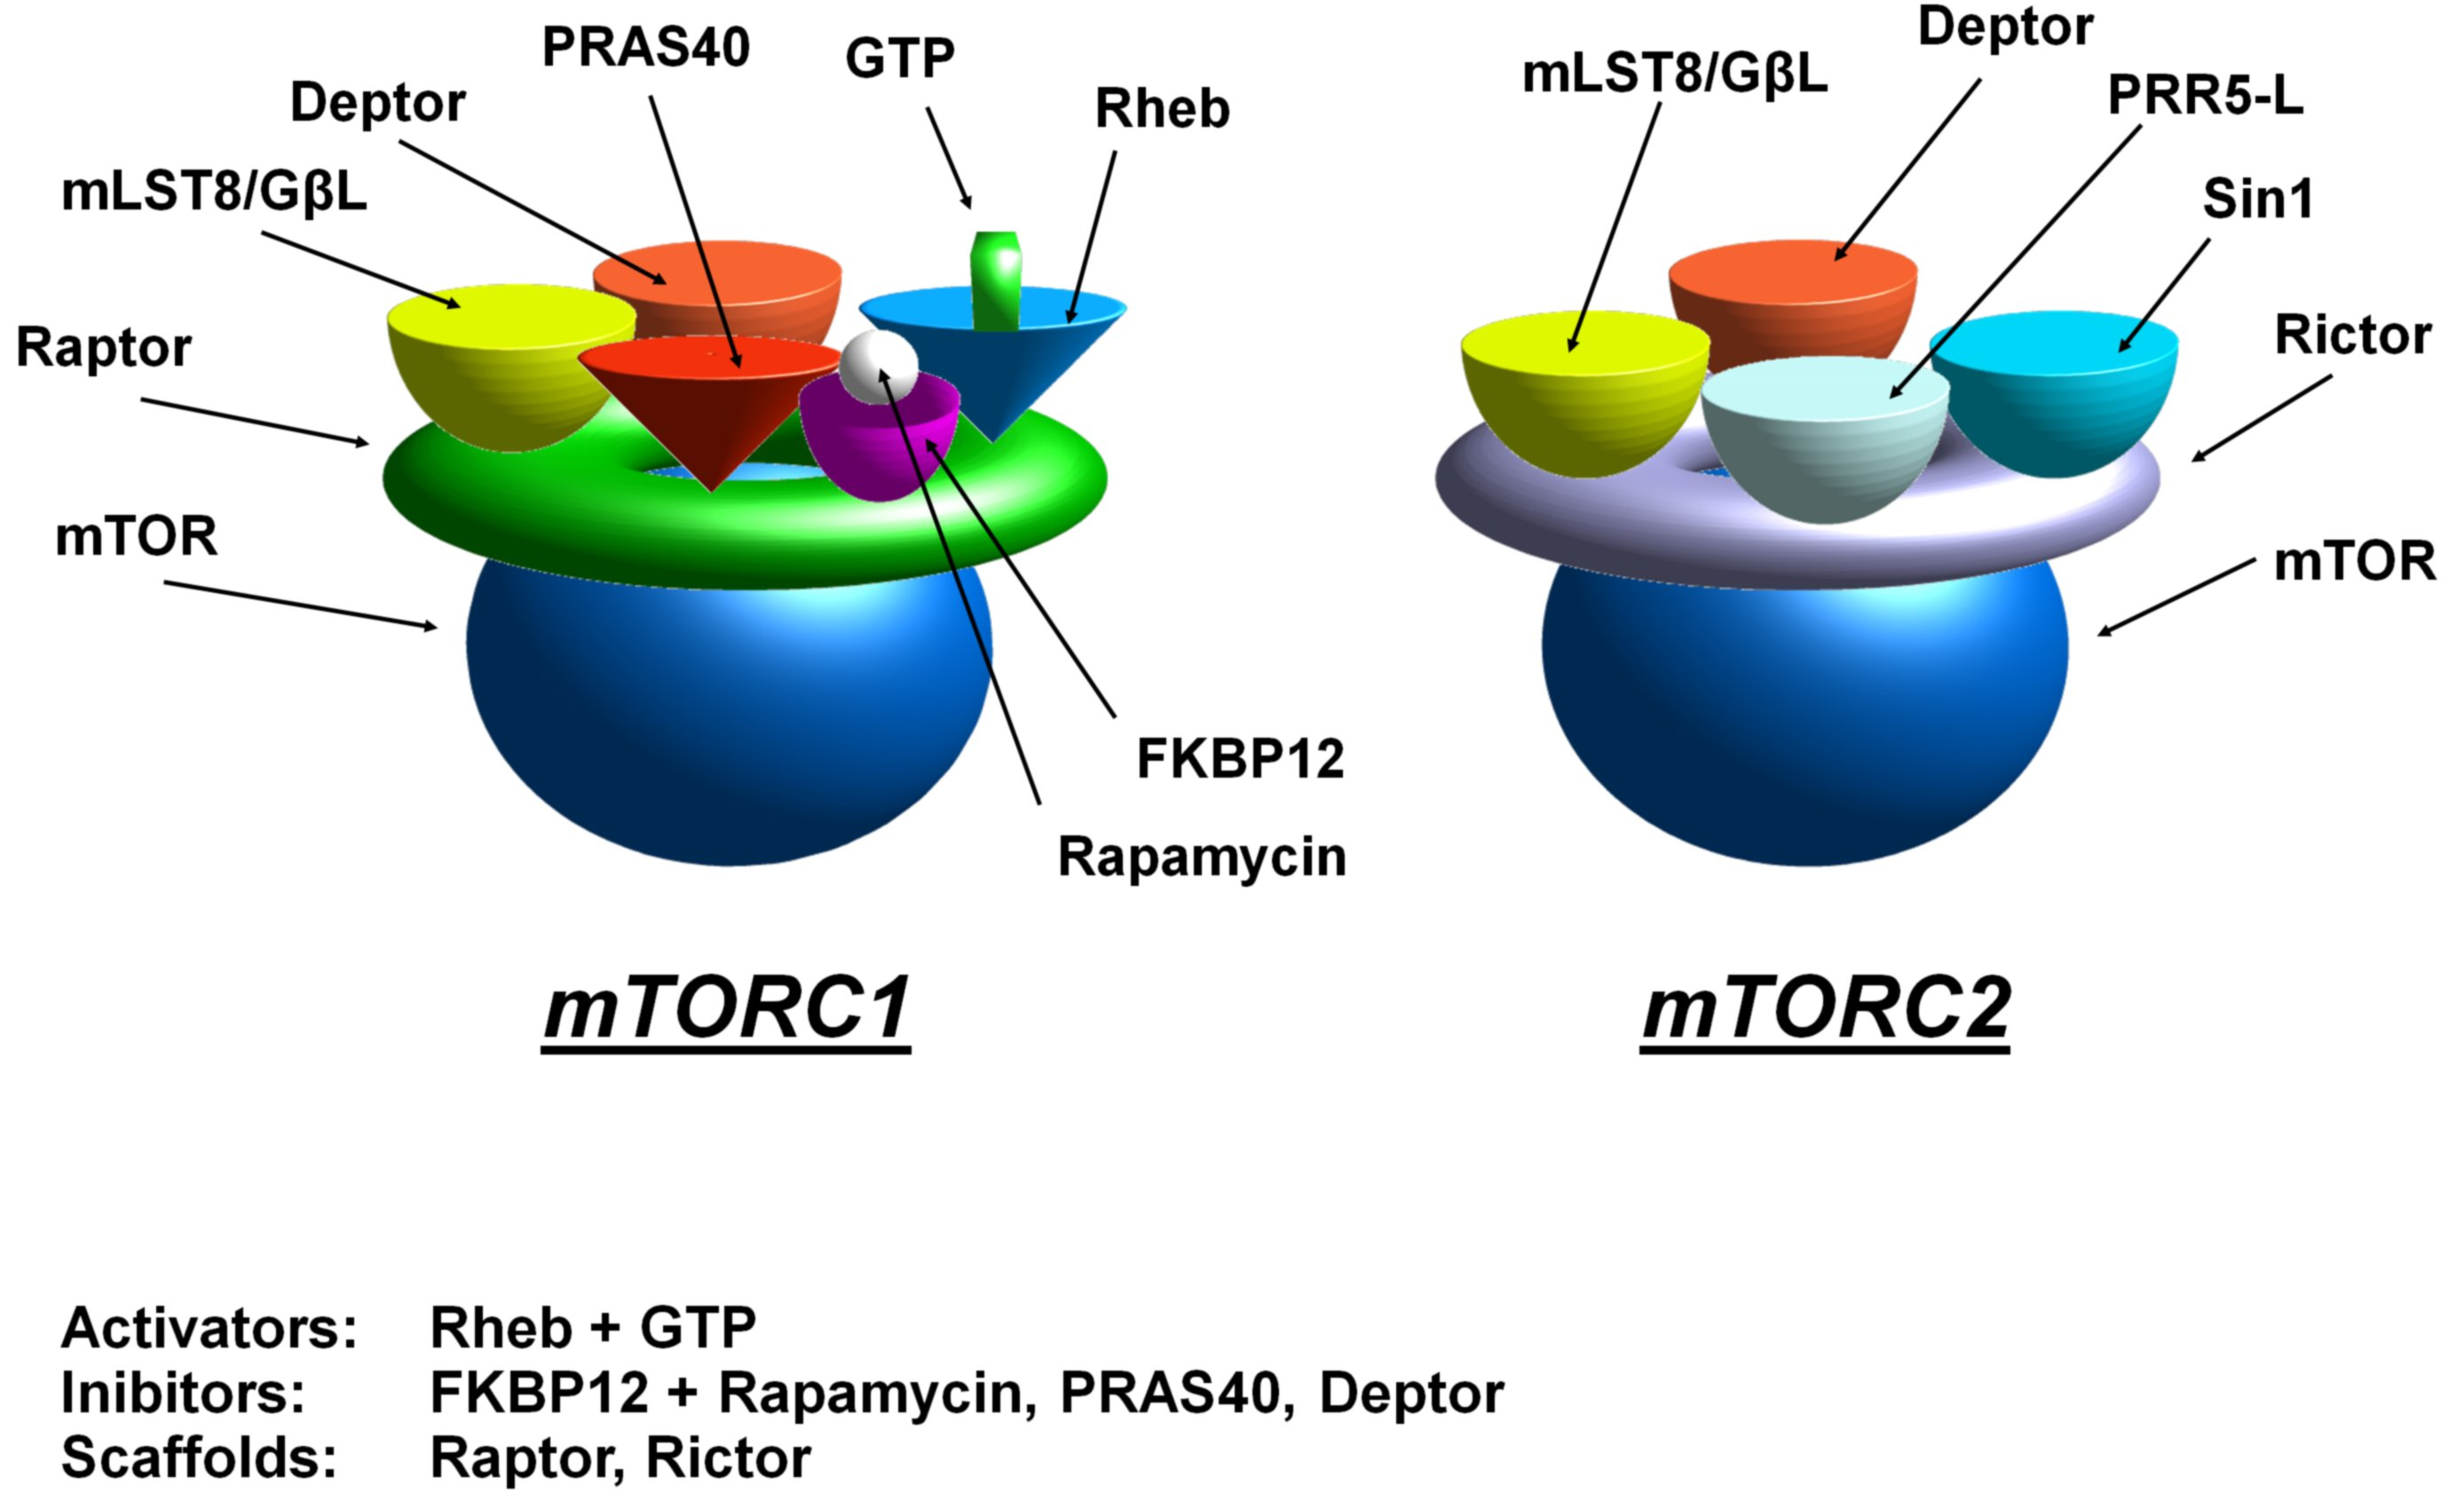
\includegraphics[scale=0.22]{mtor_complexes.jpg}
		\caption[mTOR complexes 1 and 2]{mTOR complexes 1 and 2. In mammals, the complexes mTORC1 and mTORC2 share mTOR, the mammalian LST8/G-protein $\beta$-subunit like protein (mLST8/G$\beta$L) and Deptor \citep{Peterson2009}. mLST8/G$\beta$L likely binds to the kinase domain of mTOR regulating its kinase activity. Deptor is known to have an inhibiting role in both complexes. A peculiar characteristic of mTORC1 is the binding with Raptor (Regulatory associated protein of mTOR). Raptor is known to be essential for the phosphorylation of mTORC1 downstream targets p70-S6K1 and 4E-BP1. It is supposed that it binds to the HEAT repeats of mTOR and it is sensitive to Rapamycin because it reduces its binding strength with mTOR in the presence of the drug. mTORC2 differs by containing Rictor (Rapamycin-insensitive companion of mTOR), the mammalian stress-activated protein kinase interacting protein 1 (mSIN1) \citep{Frias2006} and PRR5-L \citep{Woo2007}. mSIN1 is necessary for the binding between mTOR and Rictor, whereas 
PRR5 has not been found relevant. The detailed function of PRR5-L is still unknown.}
		\label{fig:mtor_complexes}
	\end{center}
\end{figure}
\begin{figure}[tb]
	\begin{center}
		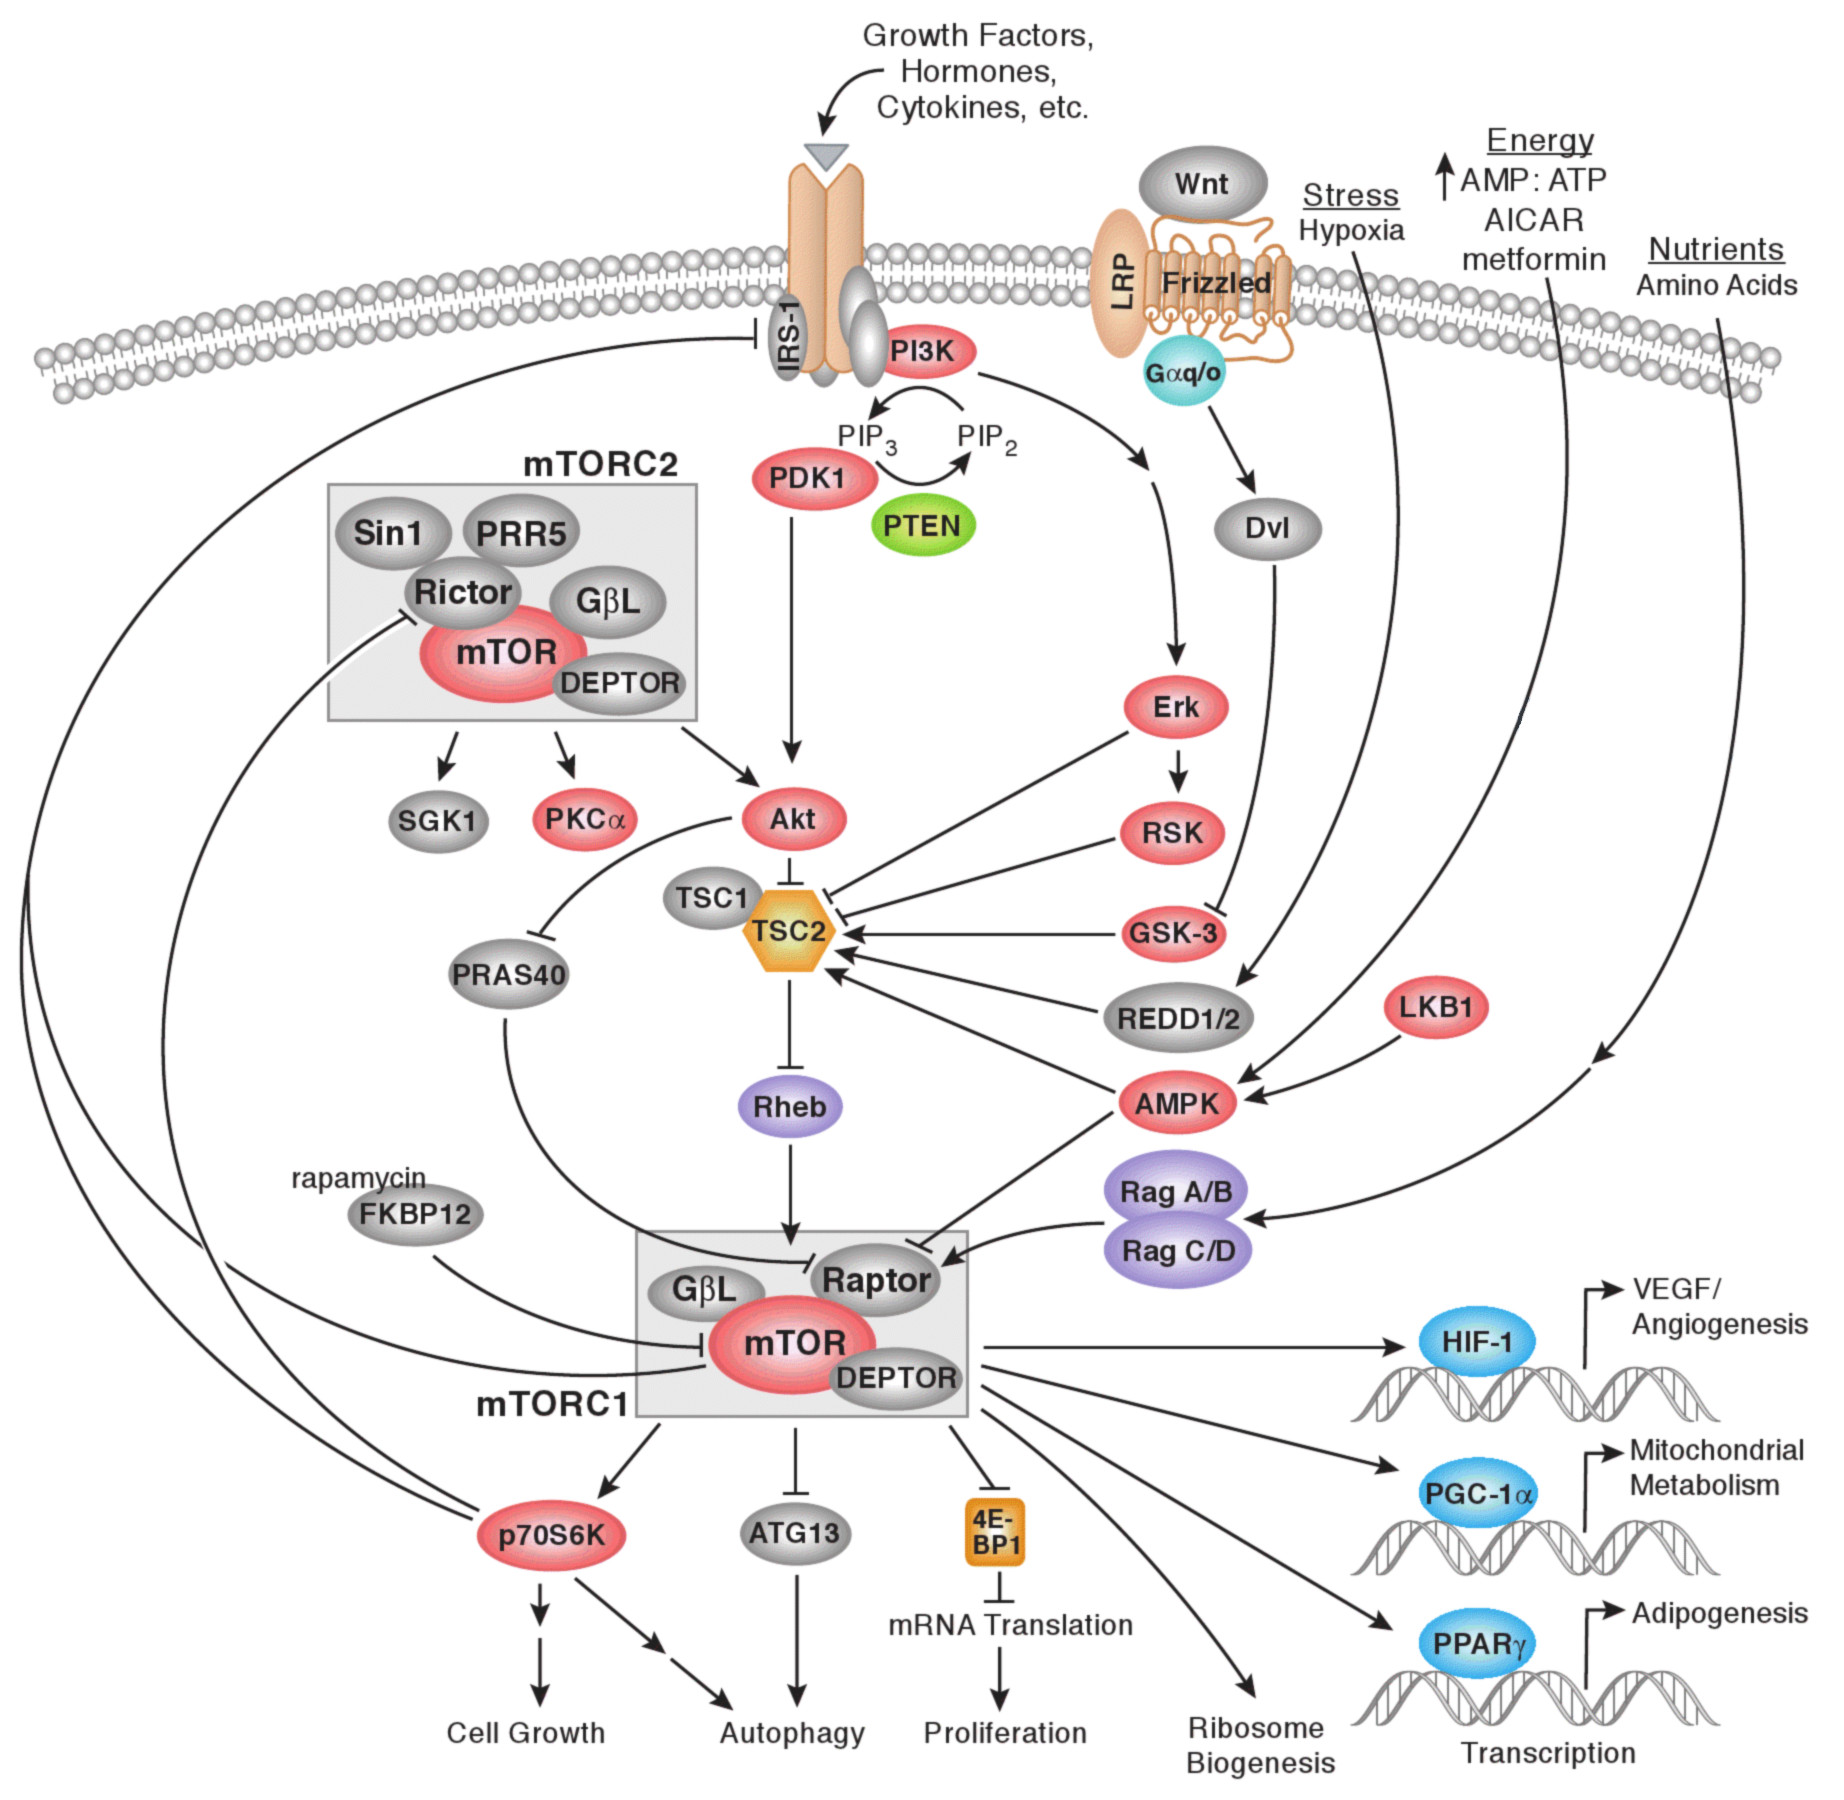
\includegraphics[scale=0.20]{mTor.jpg}
		\caption[mTOR signalling pathway]{The mTOR signalling network is complicated by the numerous inputs and interaction between signals. In addition, the network presents several negative and positive feedback loops and most of them are not completely understood. Understanding the relationships among the proteins and the mechanisms by which mTOR-dependent processes are regulated is of fundamental importance to enable intervention on numerous age-related diseases. New systems biology approaches, such as modelling, using phosphoproteomics data, are able to deal with the complexity of the network and predict both qualitative and quantitative regulations. (Source: Cell Signaling Technology$^\text{\textregistered}$ (CST), Inc., website: \url{http://www.cellsignal.com/}; proteins are linked to PhosphoSitePlus$^\text{\textregistered}$ (PSP), website: \url{http://www.phosphosite.org/} (CC BY-NC-SA 3.0) \citep{Hornbeck2012}).}
		\label{fig:mTOR}
	\end{center}
\end{figure}


\clearpage


% ------------------------------------------------------------------------


%%% Local Variables: 
%%% mode: latex
%%% TeX-master: "../thesis"
%%% End: 
